\chapter{医学知识库构建与检索方法}

本章主要研究医学问答系统中知识库的关键内容，重点包括医学知识库构建、文本语义切分、向量化表示以及混合检索策略设计。对RAG系统来说，知识库的质量和检索效果会直接影响后续生成阶段能否获得可靠证据，因此，本章重点讨论医学问答中的证据来源、知识组织方式以及检索支撑过程。

\section{医学知识库构建方法}

\subsection{数据来源}

医学知识库的数据来源，会直接影响系统问答的准确性和可靠性。围绕“三高”（高血压、高血糖、高血脂）相关内容，系统主要选取公开、并且具有一定权威性的医学资料，用来保证知识内容在科学性和可信度方面更有依据。整体来看，数据主要来自以下三个方面：

\begin{enumerate}[label =(\arabic*)]

    \item 权威医学指南与报告：主要包括国家卫生健康委员会等官方的政策文件、指南与规范和健康报告。
    \item 医疗机构与专业平台内容：主要包括丁香园、医知源等平台发布的疾病科普文章和健康建议。
    \item 医学科普网站与百科类资源：主要包括维基百科等平台中“三高”相关词条。

\end{enumerate}

\subsection{数据预处理}

本系统的医学知识库由多种格式的原始文档组成，主要包括PDF文档和HTML网页内容。由于不同来源的数据在结构上差异较大，系统针对不同类型的数据分别设计了预处理方式，先把原始文档转成适合后续处理的文本格式，再继续进行文本切分和向量化表示。
\begin{enumerate}[label =(\arabic*)]

    \item PDF文档处理：对于PDF格式的医学资料，系统使用MinerU工具进行解析。MinerU基于多模态大模型，能够识别不同排版结构的PDF文档，并把它们转换成结构化的Markdown（.md）格式。
    \item HTML网页处理：对于HTML网页数据，系统通过解析网页内容，并使用document.body.innerText提取其中的主要文本信息，再把它转换成纯文本（.txt）格式，便于后续统一处理。

\end{enumerate}

\subsection{文本语义切分}

在RAG系统中，模型通常不需要把整篇文档原封不动地作为生成时的输入，而且过长的文档还会导致向量化表示和检索的难度增加。这就要求必须对文本进行合理的切分，在尽可能保留原始医学文本语义结构的前提下，将长文档划分为适合检索与生成使用的文本块。如果切分后chunk过长，单个文本块中会包含过多无关信息，影响检索精度；若切分后chunk过短，则容易破坏上下文完整性，导致关键知识被割裂。因此，本系统切分策略并不是简单的按固定长度截断，而是要按照标题和段落结构来切分文档。

对于PDF解析得到的Markdown文本，系统会先去除文末的参考文献、页脚等与问答无关的内容，之后则按照Markdown语法识别标题与正文块。系统会创建一个标题栈，通过维护标题栈记录当前文本所在的层级路径，当遇到新的标题时，先把之前缓存的内容输出，再更新标题路径；当遇到普通段落时，则将其合并到当前标题对应的缓冲区中。如果缓冲区内容超过长度阈值，系统会优先按照句号、问号、感叹号等语句结束标点进行切分，并将上一个文本块末尾的120字符作为下一文本块的开头，从而形成带重叠的连续片段，尽量避免关键信息被分割。经过这样的处理，Markdown文本最终被切分为“标题路径+正文内容”的结构化片段。

对于网页提取得到的TXT文本，由于其与Markdown不同，并不具有“标题”和“正文”的标识，系统采用启发式规则进行语义切分，但总体的切分思路相同。程序首先按连续空行划分自然段，再对单行或多行段落进行标题识别。标题识别主要依据中文医学资料中常见的编号形式，如“一、”“（一）”“1.”“（1）” 等，同时对长度较短且不以句末标点结束的行引入隐式标题判定规则，以适应网页文本中未显式标注层级但具备标题特征的内容。与Markdown文档处理方式相同的是，系统仍会创建一个标题栈用于记录段落所属的层级关系。在具体合并策略上，若新标题属于同级或更高层级，则输出当前缓存内容并开始新的文本块；若仅为更深层级的子标题，则不立即切分，而是继续在父级主题下聚合内容。这样可以将同一主题下若干较短的小节内容合并为一个较完整的语义单元，避免切分过碎。当缓冲区长度超出阈值时，采用和之前同样的策略，按照语句结束标点切分，并且使两段又一部分重叠的片段，保留上下文的信息。

完成处理后，所有文档都统一保存为 JSON 格式，JSON字段如图\ref{fig:chunk}所示，每个文本块包含chunk\_id、source、category、headings 和 content 等字段，方便后续对检索结果的溯源。

\begin{figure}[htb]
    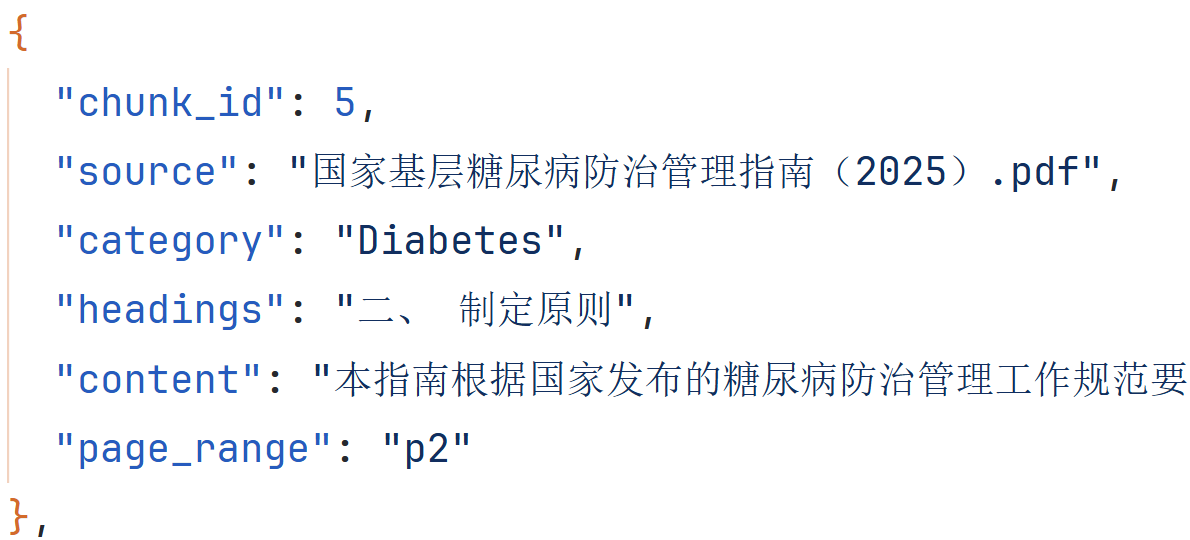
\includegraphics[width=0.7 \textwidth]{image/3/chunk.png}
    \caption{切分后的chunk示例}
    \label{fig:chunk}
\end{figure}

\subsection{Embedding向量化表示}

文本切分完成之后，知识库里的每个文本块都还需要经过一步转换，变成能够支持语义检索的向量表示。Embedding模型会把离散文本映射到一个统一的高维语义空间中，使语义相近的文本在向量空间中的距离更近，从而支持后续基于相似度的向量检索。

本系统采用BGE系列Embedding模型对医学文本块进行向量化处理。BGE模型具有较好的中文语义表示能力，能够较好地适应医学问答场景中常见的疾病名称、症状描述、用药建议以及生活化表达等多种文本形式。在知识库构建阶段，系统使用BGE模型对切分后的chunk逐条编码，生成对应的稠密向量；在在线检索阶段，则对用户问题执行相同的编码操作，并通过计算问题向量与知识块向量之间的相似度来完成召回。

Embedding向量化的意义在于，它把知识库的检索方式从单一依赖关键词匹配，转变成了兼具基于语义理解进行检索的能力；针对医学问答中大量存在的同义表达、口语化描述和隐含问题，这种向量化表示正是扩大召回覆盖面、增强检索稳健性的关键基础。

\subsection{向量数据库构建}

在获得文本块的向量表示后，还需要构建能够支持高效近邻检索的向量数据库或向量索引结构。若仅对全部向量进行线性遍历比对，在知识规模增长后会显著增加检索开销，难以满足在线问答场景对响应速度的要求。因此，知识库构建不仅包括文本组织和向量生成，也包括向量检索结构的建立。

本系统采用FAISS构建医学知识库的向量索引，把每个文本块向量与它对应的原文内容、标题路径和来源信息建立起映射关系，这样在向量检索时系统既能快速获得与查询最相近的文本块，又能把结果回溯到原始文本内容和来源元数据，为后续的证据展示与可解释性分析提供支撑。

\section{医学文本检索方法}

\subsection{BM25关键词检索原理}

BM25是一种比较经典的关键词检索模型，主要根据查询词在文档中的出现情况来计算相关性，因此更适合处理以词面匹配为主的检索任务。对于查询$q$和文档$d$，它的得分公式可以写作
\begin{equation}
\mathrm{score}(q,d)=\sum_{t\in q}\mathrm{idf}(t)\cdot
\frac{f(t,d)\cdot(k_1+1)}{f(t,d)+k_1\cdot(1-b+b\cdot\frac{|d|}{\mathrm{avgdl}})}
\end{equation}
式中，$f(t,d)$表示词项$t$在文档$d$中的出现次数，$\mathrm{idf}(t)$表示逆文档频率，$|d|$表示文档长度，$\mathrm{avgdl}$表示平均文档长度，$k_1$和$b$则用来控制词频影响和长度归一化程度。

在医学问答场景里，疾病名称、药物名称、检查指标和各类专业术语往往具有很强的区分作用，而BM25正好比较擅长保留这类关键词信息，所以在精确匹配方面表现比较稳定。它的不足也很明显，就是对同义表达、口语化提问和更深一层的语义关系不够敏感，因此只依赖BM25时，系统容易漏掉一些意思接近但表述不同的内容。

\subsection{向量检索原理}

向量检索的思路和关键词检索不同，它不是直接看词是否匹配，而是先借助嵌入模型把用户问题和文档内容都表示成向量，再放到同一个语义空间中进行比较，语义越接近，向量之间通常也越接近，系统就更容易把对应文本检索出来。本文选用BGE-M3作为嵌入模型\cite{chen2025m3embeddingmultilingualitymultifunctionalitymultigranularity}，并把知识库中的每个文本块编码成稠密向量，再写入FAISS索引中保存。

在相似度计算方面，常见方法主要有余弦相似度和内积两种形式，当向量完成归一化以后，这两种做法在效果上可以看作基本一致。结合工程实现需求，本文在FAISS中采用内积检索方式，也就是IndexFlatIP，这样既能保持较高的检索效率，也能较好反映语义层面的接近程度。

和关键词检索相比，向量检索更擅长处理同义表达、上下位概念以及长句语义理解这类问题，比如提问方式发生变化以后，它仍然有可能找到意思接近的文本。不过，它对局部关键词的约束相对较弱，有时会召回语义上看起来相关、但关键实体并不一致的文本片段。医学问答对术语准确性要求较高，所以只依靠向量检索也很难保证结果始终稳定，通常还需要和关键词检索配合使用。

\subsection{混合检索策略}

为兼顾“术语精确匹配”与“语义泛化召回”两个目标，本文采用BM25与向量检索的混合策略，并设计了一条“双路召回到融合排序再到重排精筛”的处理流程：

第一步，系统让两种检索逻辑各自独立地从知识库中检索出各自认为最相关的候选文档列表，形成两路结果；第二步，对这双路结果执行融合排序，采用的算法是倒数排序融合，它的计算形式可以写作：

\begin{equation}
RRF(d)=\sum_{r\in R}\frac{1}{k+r(d)}
\end{equation}
其中R代表参与融合的各路排序列表的集合，r(d)表示某篇文档d在对应列表中的排列位次，k是一个用来平滑结果的常数，本系统取k=60，这个公式综合了一篇文档在不同排序列表中的名次信息，名次越靠前最终得分越高；第三步，融合出统一的候选列表后，再引入BGE-Reranker-v2-M3的专门重排模型，对候选文档进行交叉编码式的高精度重排，最终截取出靠前的Top-K份证据。

与单用一种检索方式相比，混合策略有几方面的好处：第一，BM25防止了关键专业术语不会因为语义而无法被准确检索；第二，向量检索弥补了同义改写和口语表达的语义召回盲区；第三，重排模型进一步提升了最终送去给生成模型用的证据的相关性，有效滤掉那些“初看沾边但不支持直接做答”的噪声片段；这样的组合策略，在同一套检索链路里同时回应了医学问答对“高召回”和“高精度”的双重严苛要求。

\section{实验与结果分析}

为了验证不同检索方法在医学知识库中的实际召回效果，本文围绕已经构建完成的FAISS索引开展了检索实验。实验中，先从知识库里随机抽取60个文本段，再根据这些文本段的内容人工设计相关问题，每个问题都对应一个预期命中的目标文本块，只要这个目标文本块出现在前$K$个检索结果中，就记作一次命中。本文选用Recall@1、Recall@5和Recall@10作为评价指标，用来衡量系统在只返回1条、前5条和前10条候选结果时的召回能力。

实验共比较了三种检索方式，一种是基于BM25的关键词检索，一种是基于BGE向量表示和FAISS索引的向量检索，另一种是本文采用的混合检索策略，也就是先结合BM25和向量检索进行双路召回，再通过Reranker完成重排，最后给出排序结果。三种方法的实验结果如表\ref{tab:rag-recall-results}所示。

\begin{table}[htbp]
    \caption[RAG检索方法Recall@$K$对比结果]{RAG检索方法Recall@$K$对比结果}
    \centering
    \begin{tabular}{lccc}
        \toprule
        检索方法 & Recall@1 & Recall@5 & Recall@10 \\
        \midrule
        BM25检索 & 0.26 & 0.81 & 0.92 \\
        向量检索 & 0.48 & 0.81 & 0.85 \\
        混合检索 + Rerank重排 & 0.59 & 0.89 & 0.96 \\
        \bottomrule
    \end{tabular}
    \label{tab:rag-recall-results}
\end{table}

从实验结果来看，三种检索方法在不同$K$值下表现出比较明显的差异。先看Recall@1，BM25检索为0.26，说明如果系统只返回首条结果，只依靠关键词匹配很难稳定命中目标文本；向量检索的Recall@1提升到0.48，说明语义检索对口语化表达、近义改写和不完全词面匹配的问题有更好的适应能力；混合检索结合Rerank重排以后，Recall@1进一步提升到0.59，是三种方法中最高的。这说明在最靠前的排序位置上，混合检索策略更容易把真正相关的证据提前放出来。

再看Recall@5，BM25检索和向量检索都达到0.81，混合检索则提升到0.89。这说明当候选范围扩大到前5条时，单一检索方法已经能够召回大部分相关文本，但仍然会出现一定程度的漏召回；相比之下，混合检索同时利用了关键词匹配和语义匹配两类信息，又经过重排模型进一步筛选，因此在前5条结果里保留了更多有效证据。对RAG系统来说，这一点很重要，因为生成模型通常不会使用过多检索结果，如果前几条证据质量不够高，最终回答质量也会直接受到影响。

最后看Recall@10，BM25检索达到0.92，高于向量检索的0.85，这说明当候选集合进一步放宽以后，BM25在专业术语、数字指标这类关键词层面的覆盖能力会更明显，更容易把目标文本放进较长的候选列表里。不过，混合检索加Rerank重排的Recall@10仍然达到0.96，依然是三种方法中最好的结果。这说明混合检索并不是简单把两种方法拼在一起，而是在不同检索机制之间形成了比较明显的互补关系，BM25负责尽量保住专业术语、药物名称和指标数值这类关键信息不被漏掉，向量检索负责补足语义层面的相似表达，重排模型再进一步减少“看起来相关、但并不是最佳证据”的干扰。

综合来看，单独使用BM25更适合术语比较明确的问题，但对自然语言表达变化会更敏感；单独使用向量检索在语义匹配上更有优势，不过在一些依赖精确术语和细粒度实体区分的问题上，仍然可能出现误召回。相比之下，混合检索结合重排策略在Recall@1、Recall@5和Recall@10三个指标上都取得了最好结果，说明这种方法更适合医学问答场景中“专业术语精确匹配”和“自然语言语义召回”同时存在的需求。因此，本文最终选择混合检索加Rerank重排作为RAG问答系统的默认检索方案。

\section{本章小结}

本章前半部分围绕医学知识库构建与检索方法展开，介绍了知识数据来源、文本预处理、语义切分、Embedding向量化表示以及向量索引构建过程，并进一步分析了BM25、向量检索和混合检索策略在医学问答场景中的特点与差异。实验结果表明，混合检索结合重排策略在召回覆盖和结果稳定性方面表现更好，能够为后续回答生成提供更可靠的证据基础。

通过这一部分的研究，系统已经基本解决了“回答依据从哪里来”的问题，也为后续围绕RAG输入组织、Prompt设计和模型优化展开分析提供了支撑。
